\documentclass[11pt]{article}

\usepackage{a4wide}
\usepackage{mathptm}
\usepackage{xspace}
\usepackage{amsmath}
\usepackage{graphicx}
\usepackage{algorithm}
\usepackage{algpseudocode}
\usepackage{tikz}
\usepackage{tkz-graph}
\usetikzlibrary{shapes.misc, positioning}
\usepackage{listings}
\usepackage{color}
\usepackage{hyperref}
\usepackage[utf8]{inputenc}
\usepackage[T1]{fontenc}

\definecolor{dkgreen}{rgb}{0,0.6,0}
\definecolor{gray}{rgb}{0.5,0.5,0.5}
\definecolor{mauve}{rgb}{0.58,0,0.82}

\lstset{frame=tb,
  language=Java,
  aboveskip=3mm,
  belowskip=3mm,
  showstringspaces=false,
  columns=flexible,
  basicstyle={\small\ttfamily},
  numbers=left,
  numberstyle=\tiny\color{gray},
  keywordstyle=\color{blue},
  commentstyle=\color{dkgreen},
  stringstyle=\color{mauve},
  breaklines=true,
  breakatwhitespace=true,
  tabsize=3
}
\begin{document}

\title{Thorntail Microservice Evaluation Project}

\author{Simon Halvorsen, Øystein Follo and Runar Serigstad}

\maketitle
\frontmatter
\begin{abstract}

\noindent This is a report about what the Thorntail framework is, what it was like working with it, and the solutions we built using it. The prototype we built during this project was a microservice based system for keeping track of available offices at Western Norway University of Applied Sciences. We will also introduce you to the tasks and challenges we were given and what role Thorntail played in this. Finally, we will do an analysis and a comparison between Thorntail, Glassfish and Spring Boot so we can help you understand what kind of framework you may want to use in your own projects. It is worth mentioning that Thorntail is still somewhat new to the software world while the technology we’re comparing to has been around since 2005 (Glassfish first release) and 2003 (Spring first release), Thorntail had their first alpha release in 2016 (then called Wildfly Swarm).

\thispagestyle{empty}
  
\end{abstract}

\newpage
\tableofcontents
\thispagestyle{empty}
\newpage
%\input{commands}
\setcounter{page}{1}
\section{Introduction}
\label{sec:introduction}

\subsection{Motivation}
The motivation for using microservices is that it provides an easy way to deploy and scale your applications, makes your codebase smaller and easier to maintain while also adding a layer of resilience inherited from the microservice pattern. This is something that is heavily sought after in the enterprise industry as trying to keep the codebase up to date, tested and then deployed can be a very difficult task once the project starts to grow in size as it eventually becomesr impossible to have insight and overview over the entire project. This is the motivation Thorntail is working with as their framework is made to build microservice applications on top of.

\subsection{Thorntail's History}
Thorntail (then called Wildfly Swarm) had their first alpha release in January 2016 and is based on Wildfly which is an application server started by JBoss in 1999 and then renamed to Wildfly in 2014. Somewhere between 2014 and 2016 (this is based on when they first started blogging about Wildfly Swarm and when they had their first public alpha release [3]), RedHat decided to branch off from their application server and create Wildfly Swarm which uses a reconstruction of Wildfly to create what is called just enough application server. This means that Thorntail is actually just a fraction of the original application server Wildfly and the idea is that you don’t want to load the entire application server with all of its modules every time you start your server when you’re creating microservices. Since then Thorntail has focused on shaping their technology more and more towards being an open source microservice framework free for everyone to use. \cite{ThorntailAnnouncement}

\subsection{Related Technologies}
As Thorntail has a lot in common with Spring Boot they have created a dependency that allows you to build traditional Spring projects within your Thorntail project allowing developers to take advantage of both frameworks within the same project. We started using this Thorntail fraction for our frontend microservice, but due to the time limitations, we didn’t get to finish it.

\subsection{Results}
The results of our project show that Thorntail is very much comparable to Spring Boot and that they’re both trying to solve the same problems, but Spring Boot is a more mature and documented framework proven by the age of the two frameworks as well as the number of search results Google yields (230 000 for Thorntail and 559 000 000 for Spring Boot). We have also found that configuring, deploying and running microservices can be a lot easier than configuring and deploying full application servers, but the different microservices require more preplanning and overview than what was required when making using an application server.
\newpage
\subsection{Article Overview}
In this report we will focus on planning, creating and deploying microservices specifically with Thorntail. The first section~\ref{sec:background} we will go in-depth about the microservice architecture, what Thorntail is and what it contains, then the next section~\ref{sec:prototype} we will go into detail about our very own prototype, what we built and how it all went. Section~\ref{sec:experiments} aims to compare the microservice architecture with more traditional architectures and finally in section~\ref{sec:conclusion} we will reveal our final conclusion using our findings and the comparisons we made in the earlier section.

\newpage
\section{Technology}
\label{sec:background}

In this section we will go into detail about microservices architecture and how we used Thorntail to achieve this. We compare a microservice architecture to a traditional monolithic approach, to look at what you as a developer and your application can benefit from choosing a microservice architecture.

\subsection{Microservice Architecture}
The idea behind a microservice architecture is to split an application into a set of smaller, interconnected services. Each microservice functions as a small application and has its own architecture consisting of business logic and a communication technology. \\

\noindent One of the most prominent features of the microservice architecture pattern is how it affects the relationship between the application and the database. In a monolithic architecture its traditional to share one database schema across the entire application, but with microservices each service has its own database schema. This will probably lead to some duplication of data across the entire application, but it's necessary to ensure loose coupling between services. \\

\noindent Another important aspect of this architecture is that client applications don’t directly communicate with the back-end services. Instead clients requests/sends information from/to an API Gateway. The API Gateway is responsible for tasks such as load balancing, caching, access control, API metering and monitoring. \cite{MicroArticle}\\

\noindent A traditional monolithic architecture usually consist of a database, application back-end and client-side. Where most of the business logic is implemented in the back-end, all the data for the entire application is stored in one database schema and the client-side requests information directly from the back-end or a REST-api. At the beginning of the development phase this is easy to develop, deploy and scale, but as time goes this can change due to increasing complexity and code base. One of the biggest drawbacks for the monolithic architecture is that it usually means a long-term commitment to a technology stack. \cite{MonolithArch}

\subsection{Concepts}
The concepts focused on in this section is what is what a microservice architecture can do for the application and its developers in the long run. Even though the microservice architecture in the {figure above} seems far more complex than the monolithic architecture, we will do our best to show that the microservice approach brings a lot of benefits to both the application as a whole and its developers. \\
\newline
Each service should be independent of the rest of the system, and have its own database. The relative small codebase for each service makes the maintenance easier, and new developers will use less time to get an understanding of the codebase which he/she is working with. \\
\newline
Scalability in a microservice architecture is also worth mentioning. The fact that you can scale up one service at the time to reduce the response time for the system is also a major benefit to the monolithic approach, where you have to scale up the entire system. In other words, you can reduce the amount of overhead you have, and it ’s more cost efficient if you are looking at server costs.\\
\newline
In a monolithic application, you have to be aware that changes in some parts of the code can affect the entire codebase. On the other hand, when you want to expand a microservice application you severely limit the implications on the whole code base when you are changing a service, or adding a new one. \cite{MonolithArch} \\
\subsection{Thorntail}
Thorntail is a framework for creating small, standalone microservice-based applications, and is based on the WildFly Java application server. It claims to offer an innovative approach to packaging and running Java EE applications by producing just enough app-server. It does this through defining fractions[7] in the application’s pom.xml file. This ensures that the executable JAR doesn’t contain more functionality than it needs. \cite{ThorntailDoc}

\subsubsection{Uber- and Hollow JAR}
Thorntail offers two types of JARs. The uberjar is a single JAR file that includes everything you need to run your application. This includes both selected runtime components and the application components. This type of jar can be used for projects with continuous integration and continuous deployment pipelines, where a single executable binary artifact is produced and moved through the pipeline. The hollow JAR, on the other hand, removes the application components from the uberjar. This is meant for applications running on Linux containers such as Docker. When using containers you can add the runtime components to a container image below the application image in the hierarchy, this means that you can rebuild the application image faster if code changes appear.\cite{ThorntailDoc} 

\subsubsection{Logging}
Thorntail automatically enables logging through each of its fractions. This means, that by default you'll get logs that are service independent. Its also possible to define custom logging patterns in the \textit{project-defaults.yml}, as described in figure~\ref{fig:logging}. \cite{Thorntaillogging}\\

\begin{figure}[ht]
  \centering
  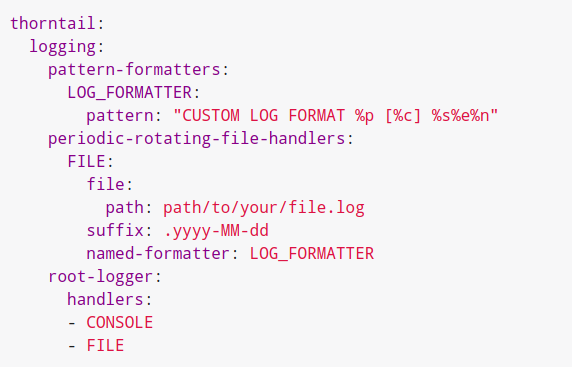
\includegraphics[scale=0.8]{figs/loggingconfig.png}
  \caption{Custom logging pattern to file}
  \label{fig:logging}
\end{figure}

\subsubsection{Distributed Tracing}
Thorntail makes it easy to debug through a process known as distributed tracing, even though an application is spread across multiple servers or instances. This is made possible through MicroProfile OpenTracing (cite something here), or another popular fraction, Jaeger (cite jaeger here). These APIs collects information about service invocations, correlating it to find all invocations related to a single user request, and visualizing the data in a form that enables easy debugging. This is also configurable through the \textit{project-defaults.yml} file in each service. \cite{ThorntailTracing}

\subsubsection{Metrics}
With this type of architecture, where a single user request invokes multiple services, diagnosing performance issues or reacting to service outages might be hard. Thorntail provides a fraction for providing metrics, namely MicroProfile Metrics. \cite{ThorntailMetrics} This enables developers to have information about:

\begin{itemize}
    \item How many requests are currently being processed
    \item How many connections to the database are currently in use
    \item How long service invocations take
\end{itemize}



\newpage
\section{Demonstrator Prototype}
\label{sec:prototype}

\subsection{The Prototype}
The prototype we built as our project was a microservice based Java EE application for keeping track of available offices at Western Norway University of Applied Sciences. The application architecture was inspired by the model-view-controller architectural pattern, but the prototype is currently lacking the view component. We implemented three independent microservices (models) which, together with a controller/gateway (controller), constitute our prototype. 

\subsubsection{Functionality}
Due to limited time, we were not able to implement all of the components we decided on initially. We decided on implementing the model and controller components so that we would have a working backend. For testing, we decided to use postman to simulate client requests that eventually will be generated by user interaction, and sent from a front end service.  \\
\newline
The prototype includes the following functionality:
\begin{itemize}
    \item Create user
    \item Mark an office as available
    \item Update office information
    \item Create new offices
    \item Book an available office
    \item Get a list of available offices, and the period they are available for
    \item Authenticate a user requesting a resource
    \item Generate session tokens
\end{itemize}

\subsubsection{Project Architecture}
Our system design, as seen in figure x (replace x with fig. num), consists of three services and a gateway/controller. The controller serves as an entry point for user requests. Its main purpose is to forward requests to the appropriate service and return the response to the client. The controller decouples the services from the clients so that the services can be updated or refactored without having to update all clients. We also built three independent and loosely coupled services implementing the business logic, each with their own database so that they can persist their own data. The purpose of the services is to process client requests forwarded by the controller and return a response. The controller communicates with the services through REST APIs, where data is sent as headers.

\begin{figure}[ht]
  \centering
  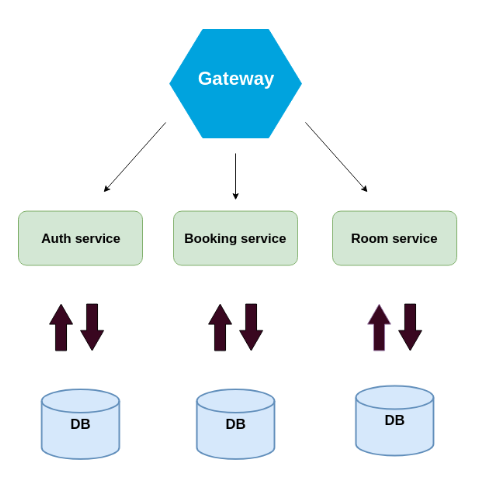
\includegraphics[scale=0.8]{figs/projectArchitecture.png}
  \caption{Project Architecture}
  \label{fig:projectarch}
\end{figure}
\newpage
\subsubsection{The Development Process}
One benefit of the architecture we had decided on, is that the services could be independently developed and tested since the services don’t depend on each other. The services were “bound” together by the controller, resulting in a pretty complex system compared to if we would have implemented the same system as a monolith. A monolithic architecture would have been easier to implement, but at the cost of independent components. Our motivation for this project was to research microservice technologies, so that is what we went with. \\
\newline

\noindent Since Thorntail is a framework for developing enterprise Java applications, we had the opportunity to use some of the same frameworks and APIs we used when developing the auction application. We decided to continue using the framework JAX-RS, to set up our REST communication, and the API JPA, for object-relational mapping. We also decided that each microservice should persist their own data in an embedded H2 relational database. 


\subsubsection{Getting Started}
Thorntail provides a project generator which generates a maven project for you based on the dependencies you choose (fig. x) at: \hyperref[https://thorntail.io/generator/]{https://thorntail.io/generator/} \\

\noindent You have the opportunity to add only the dependencies you need or none at all. The maven plugin also auto-detect dependencies added during the development process, so you don’t need to know exactly what dependencies you are going to need when starting a project.

\begin{figure}[ht]
  \centering
  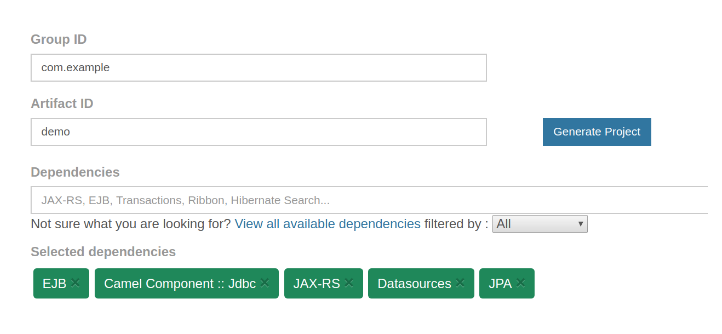
\includegraphics[scale=0.7]{figs/thorntailgenerator.png}
  \caption{Thorntail Generator with selected dependencies}
  \label{fig:thorntailgenerator}
\end{figure}

\subsubsection{Database}
In our application we needed each microservice to store the application data, and the authentication service to keep track of session tokens. As for how to store the data, we went with embedded H2 databases. To set up a H2 database, all we had to do was to configure the datasource in the project-defaults.yml file as seen in figure x.\\

\begin{figure}[ht]
  \centering
  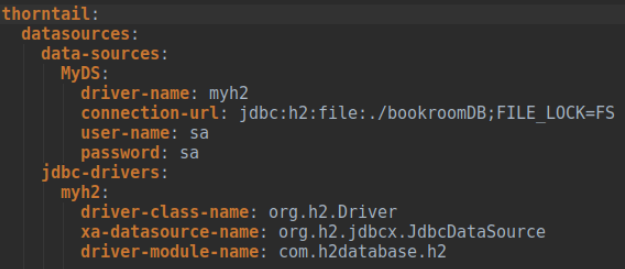
\includegraphics[scale=0.9]{figs/databaseconfig.png}
  \caption{Database Configuration}
  \label{fig:databaseconfig}
\end{figure}
\newpage
\noindent A new, empty database will be created if the database specified in the URL doesn’t exist. The mapping between the databases and the application objects is defined by persistence metadata. In our project, the JPA metadata is defined by annotations and used to perform different database operations. In this way, we were able to work with the objects of our system, instead of writing SQL statements. The javax.persistence.Entity  (beautify in latex) annotation makes an entity class, and \textbf{javax.persistence.Column} defines the columns of the tables. JPA will create tables in the database corresponding to the persistence metadata. The \textbf{javax.persistence.EntityManager} provides four basic operations of persistent storage that we made use of in our project:

\begin{itemize}
    \item Persist, to add new objects to the database
    \item Find, to find and return an object/objects
    \item Merge (edit), to update an object
    \item Remove, to delete an object
\end{itemize}

\noindent The persistence.xml describes the persistence unit, and the persistence unit configures the EntityManager. The EntityManager instance manages the entities by using the PersistenceContext, and it can be injected via the \textbf{@PersistenceContext} annotation, as shown in figure x. Entity instances and lifecycles are managed within the scope defined by the PersistenceContext. The EntityManager serves as a reference to the PersistenceContext associated with a transaction. The PersistenceContext is pretty much a cache which contains a set of persistent entities. When a transaction is committed, the persistent objects are detached from the PersistenceContext, and it is flushed and cleared.\\

\begin{figure}[ht]
  \centering
  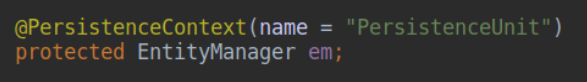
\includegraphics[scale=0.9]{figs/persistencecontext.png}
  \caption{PersistanceContext}
  \label{fig:databaseconfig}
\end{figure}

\newpage

\subsubsection{Communication}
The services in our prototype communicate with the controller using rest APIs. Each microservice has its own rest API with endpoints triggered by incoming requests from the controller. Figure x shows an example endpoint from the authentication service that is triggered when a session token needs to be verified. This method returns a boolean value to the controller, letting it know whether the token is valid or not. \\

\begin{figure}[ht]
  \centering
  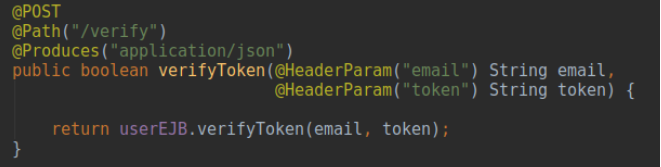
\includegraphics[scale=0.9]{figs/verifyendpoint.png}
  \caption{Verify Endpoint}
  \label{fig:databaseconfig}
\end{figure}

\noindent Triggering this endpoint will call the backend logic for verifying a user’s token, shown in figure x. The method fetches the user with given email from the database or throws an exception if the user doesn’t exist. If the user has an active session, i.e. \textit{user.getAuthToken()} does not return null, the stored session token it is matched against the token that came with the request. If they are identical, the user will be verified, otherwise, the user will not be verified.  

\begin{figure}[ht]
  \centering
  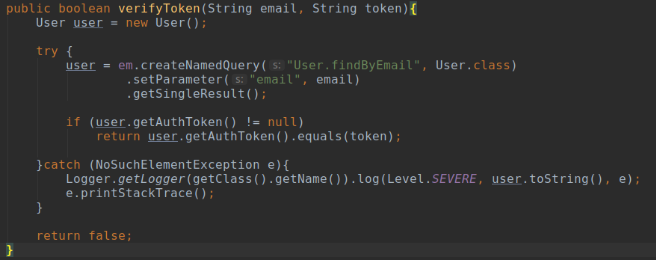
\includegraphics[scale=0.9]{figs/verifytoken.png}
  \caption{Verify Token}
  \label{fig:verifytoken}
\end{figure}
\newpage
\noindent The endpoints in the controller are triggered by incoming user requests. When a client requests a resource, the controller opens an HTTP connection to the appropriate resource’s URL, sends a POST request with the headers from the incoming request, and fetches the answer from the service. Figure x shows a method for sending requests and fetching a response from the controller, taking an URL and headers as parameters. The fetch will either return a response or null if there was an error, in which case it will Log a warning with the response code. \\

\begin{figure}[ht]
  \centering
  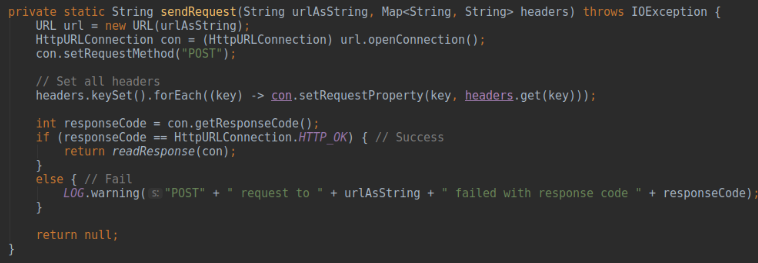
\includegraphics[scale=0.75]{figs/sendrequest.png}
  \caption{Send Request}
  \label{fig:databaseconfig}
\end{figure}

\noindent An example of session token verification is shown in figure y. The controller sets the headers to match the corresponding headers of the incoming client request, i.e. email address and session token and sends it using the method in figure x. The verify method will return the result from the sendRequest method. This means that triggering the verify endpoint will result in either true (valid), false (not valid), or a connection error.\\

\begin{figure}[ht]
  \centering
  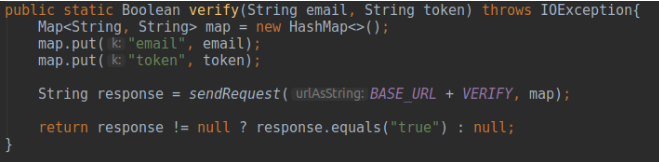
\includegraphics[scale=0.75]{figs/verify.png}
  \caption{Verify}
  \label{fig:databaseconfig}
\end{figure}

\noindent Throughout the whole system, requests are sent and processed in a similar manner as explained above. The only difference between requests is features specific to each request, such as the URL of the resource endpoint, and which headers to send with the request. Responses are also requested specifically. A successful log-in, for instance, will return a session token, while the session token verification returns a boolean. As mentioned earlier, the controller controls the flow of requests and forwards them to the appropriate backend service, where the requests are processed, and a proper response returned to the controller. 

%\lstinputlisting[language=java]{code/BoksVolum.java}

\newpage
\section{Test-bed Environment and Experimental Results}
\label{sec:experiments}

\subsection{Planning and Design}
The first thing we noticed was that the microservice architecture required more careful planning as we needed to know exactly what kind of microservices we would need before we could even start working on the project as well as we had to find a common way we could communicate between our different services. While the Glassfish Java EE application had to design and plan data structures, security and client-server communications the microservice application had to design and plan all of this in addition to the previously mentioned preplanning. This meant that our microservice application required additional design time before we could start the actual development of our application, but it also meant that we already knew who would be working on what service and what role that service would play in the application before we had even begun writing a single line of code.

\subsection{Initial Setup and Configuration}
Due to the nature of microservice architecture the frameworks built for this kind of architecture has all the required configuration inside the source code of the application, while the traditional monolith application will have the server configuration put inside the application server running the source code, this means that setting up the same server running locally on our three different machines required us to make sure we were all running the exact same version of the application server and that we all had the exact same configuration setup. The initial setup for Thorntail was very simple, they gave us a generate button on their website that generated the initial configuration, folder structure and dependencies we needed to get a kick-start to our project while Glassfish was a lot more researching the documentation and reading up on configuration then testing and trying until you got it to work on your computer then tell everyone else on the group to attempt to do exactly the same as you just did.

\subsection{Development}
The largest difference between developing with a microservice architecture compared to a monolithic architecture was that each one of us worked with our very own project, we were each our own team and instead of programming together we were simply communicating together, this meant that we all had an individual GitHub repo and we could be much more free on how we developed our service. When building the Java EE Glassfish server we had all of our different java classes and structures all put into one single project which quickly made it messy, especially since we had SOAP endpoints, REST endpoints, and normal XHTML endpoints all built into the same application, when we instead could’ve built one microservice for each of these different endpoints, it would’ve kept the project structure a lot simpler and made it easier to work with. It seemed to us that a big company could benefit from using microservices by dividing each microservice into a more tightly coupled team of developers that then communicates with the other teams, that way they could each choose their own technology that best suits their needs. The largest problems we encountered during the development process while using the microservice architecture was when a team updated their endpoints without announcing it to the other teams that were using their endpoint in their service, this meant that breaking changes to the endpoint had to be fixed in every service that used them.

\subsection{Deployment}
Thorntail made deploying all our different services simple as the only requirement to run the application is to have the correct version of Maven and the Java JDK installed, then all we had to do to start the application was to run a terminal command
\begin{lstlisting}[language=bash]
  $ mvn thorntail:run
\end{lstlisting} or
\begin{lstlisting}[language=bash]
  $ java -jar thorntailservice.jar
\end{lstlisting} if the project had already been compiled to a jar file. When deploying the Glassfish server you were required to have the correct version of Glassfish and the Java JDK installed as well as the correct configuration before you could run the command 
\begin{lstlisting}[language=bash]
  $ asadmin start-domain
\end{lstlisting}, then 
\begin{lstlisting} [language=bash]
  $ asadmin deploy <.war location>
\end{lstlisting}
and if you wanted a local database you also had to run the command 
\begin{lstlisting}
  $ asadmin start-database
\end{lstlisting}
, while the Thorntail command started everything for you.

\subsection{Response Time}
We performed a response time test of our microservice application by running HTTP requests to a specific endpoint in the controller and then printing the time it took to get a response for the request. After testing the microservice application we tested it as a monolith application by running the same request to the equivalent endpoint directly to the service itself instead of going through the controller. Below is the response time (in ms) for our login endpoint when set up as a microservice and when it’s set up as a monolith. \\

\begin{table}[ht]
\centering
\begin{tabular}{ccc}
  Request# & Microservice & Monolithic
  \\ \hline
1 & 557.321  &    101.522 \\
2 & 92.327   &    57.58 \\
3 & 553.268  &    22.909 \\
4 & 147.223   &    49.168 \\
5 & 131.688   &    71.541 \\
6 & 93.646   &    120.513 \\
7 & 73.144   &    85.397 \\
8 & 139.275   &    61.725 \\
9 & 127.242   &    72.325 \\
10 & 72.602   &    32.835 \\
\hline
Sum & 1987.736   &    675.515 \\
Avg & 198.7736   &    67.5515 \\

\end{tabular}
\caption{Selected experimental results on the communication protocol example.}
\label{tab:results}
\end{table}

\noindent You can see from the table~\ref{tab:results} that the response time has been significantly increased by using microservices, but as a reader you need to be aware that this data is exaggerated due to the fact that we ran the tests while the client was connected to the same network as the server (and everyone ran a wireless connection), but in most real cases you will be connected to a server in the cloud or at least a server in a different area which would make the average 131ms difference a lot less significant compared to what it looks like here. It is also worth mentioning that our servers were running on common student laptops and not a dedicated server. Due to these factors playing an important role in the results above we can only conclude that our microservice will take longer time responding to a request compared to what our monolith application does, but we can’t know for sure how large the difference in response times will be when our application is fully deployed. Our assumption is that the difference in milliseconds will lower quite a lot as a dedicated server directly connected to its services will lower the time it takes for the controller to send a request to the correct service and that the HTTP overhead will play a more significant role than it did during our tests.


\section{Conclusions}
\label{sec:conclusion}

This report compares Thorntail microservices to monolithic Glassfish Enterprise Java, this does not necessarily mean our comparison between microservices and monolithic systems is fair, but overall it still gives good insight into the differences between the two architectures and our experience working with Thorntail and Glassfish. Since we only had time to create our project using one framework for microservices and one application server for the monolithic application we can’t speak for all microservice technologies and all monolithic technologies it means our experience within these architectures will be highly coherent with the technology and not just the architectures alone. \\

Dividing the system up into several different projects made it easier for everyone to find their own solution and build with the tools they felt most comfortable with, it made it easier to assign people to different roles such as frontend developer, database administrator and backend developer. It also changed the way we communicate as we no longer cared about the technology and dependencies the other teams had used in their project as long as we all stayed with the same communication methods, this meant that we would ask more questions like “Can you give me an example request for how to create a new user?” instead of “How do you create a new user?”, the questions may look pretty similar, but the answer to the first question results in an example answer, whereas the second question often resulted in being given the name of the source file where we create new users.\\

Thorntail has a lot easier initial setup and are easier to deploy compared to the Glassfish server, this is most likely due to the fact that microservices require you to go through the initial setup multiple times and whenever you want to deploy the entire application you have to deploy every single service once each which means that microservice frameworks are forced to make this experience as fluent and easy as possible. Glassfish was a lot harder to initially set up, configure and deploy, but monolithic applications only have to do the initial setup once and deploy much less frequently so the aspect is much less important in this kind of application.\\

Microservices have longer response times than monolithic applications, this is due to overhead and connection times of each service as they all have to communicate together to perform the tasks the client asks for, this means that a single request from a client can result in the server sending out several different requests to different services which then has to wait for a reply from the services before it can then reply to the client. A monolithic system will simply do all of these actions internally which means no overhead and no additional connection times.\\

The final conclusion from this project is that microservices are a great way to divide up large enterprise systems into much smaller and more manageable projects that can be easily set up, configured, deployed and tested, but it’s not always worth all the extra planning and required monitoring when developing smaller systems like the one in our project, but it can still be worth using microservice technology and frameworks even if you’re not going to follow the microservice architecture just simply because of the simplicity in configuration and deployment. This means that smaller systems and projects should use microservice technology if possible, but not necessarily follow the architecture.\\

\newpage
\bibliographystyle{plain}
\bibliography{report.bib}{}

\end{document}
